This chapter presents background information on virtualization and confinement
technologies in Linux and other Unix-like operating systems. It also presents a detailed
history and examination of eBPF and discusses its applications in the domains of computer
security, performance monitoring, and beyond.

\begin{comment}
\section{Virtualization Technologies}%
\label{s:virtualization-bg}

\subsection{Namespaces}%
\label{ss:namespaces-bg}

\subsection{Process Control Groups}%
\label{ss:cgroups-bg}

\subsection{Hypervisors and Virtual Machines}%
\label{ss:vms-bg}




\section{Confinement Technologies}%
\label{s:confinement-bg}

\subsection{FreeBSD Jails}%
\label{ss:jails-bg}

\subsection{OpenBSD Pledge and Unveil}%
\label{ss:pledge-bg}

\subsection{Linux Seccomp and Seccomp-BPF}%
\label{ss:seccomp-bg}

\subsection{Unix DAC}%
\label{ss:unix-dac-bg}

\subsection{Linux MAC}%
\label{ss:linux-mac-bg}




\section{Linux Containers}%
\label{s:containers-bg}
\end{comment}




\section{Extended BPF}%
\label{s:ebpf-bg}

eBPF stands for \enquote{Extended Berkeley Packet Filter}, though in reality it has very
little to do with Berkeley, packets, or filtering in its current form.  In a nutshell,
eBPF is a Linux kernel technology that supports dynamic monitoring of a production system
through the attachment of special \enquote{hooks} called BPF programs to specific kernel
interfaces and userspace functions. In this section, we discuss the origins of eBPF, its
components and how they work, its applications under the Linux kernel, and how it has
evolved over time.

\todo{Perhaps add a subsection here to discuss DTrace as a precursor to eBPF?}

\subsection{Origins of BPF\@: Efficient Packet Filtering and Beyond}%
\label{ss:origins-of-bpf-bg}

The original Berkeley Packet Filter, hereafter referred to as classic BPF or
cBPF\footnote{Throughout the rest of this thesis, we refer to extended BPF using the terms
\enquote{eBPF} and \enquote{BPF} interchangeably. This is a matter of established
convention within the eBPF community. Classic BPF will be explicitly referred to by its
full name or the cBPF acronym.}, arose out of a need to implement a more efficient packet
filtering mechanism for BSD Unix.  McCanne and Jacobson~\cite{mccanne1993_bpf} published
their work on cBPF in 1993, marking an improvement over existing mechanisms in a number of
ways. Many of the reasons why classic BPF was such an improvement over the status quo are
still relevant when discussing \textit{eBPF}, and so we will briefly cover them here as
well.

In essence, classic BPF is a \textit{register virtual machine} designed to take packets
as input and produce \textit{filtering decisions} as output. These filtering decisions
could then used to make decisions about whether a packet should be passed down to a more
complex pipeline for further analysis. The key insight behind classic BPF is that these
filtering decisions could be made more efficiently in \textit{kernelspace}, the part of
the operating system that runs in protection ring 0\footnote{In practice, ring 0 is the
highest real level of memory protection offered by the CPU (although negative rings do
exist on modern CPUs, they are, in fact, merely partitions of ring 0)~\todo{CITE}. Code
that runs in ring 0 is said to run with \textit{supervisor privileges}.} and which is most
commonly associated with any parts of the operating system that do not run in
\textit{userland} (i.e.~the context of an ordinary user process). This provides
a considerable performance advantage over conventional approaches to network monitoring.
A typical network monitor runs in \textit{userspace}, meaning that packets need to be
copied over from kernelspace before they can be properly analyzed. This is an expensive
operation, requiring several context switches and potentially sleeping in the event of
a page fault~\cite{mccanne1993_bpf}. By applying filtering logic in the kernel, this
expensive copying could be skipped for packets that would be discarded or ignored by the
network monitor anyway.

\begin{figure}[tbp]
  \centering
  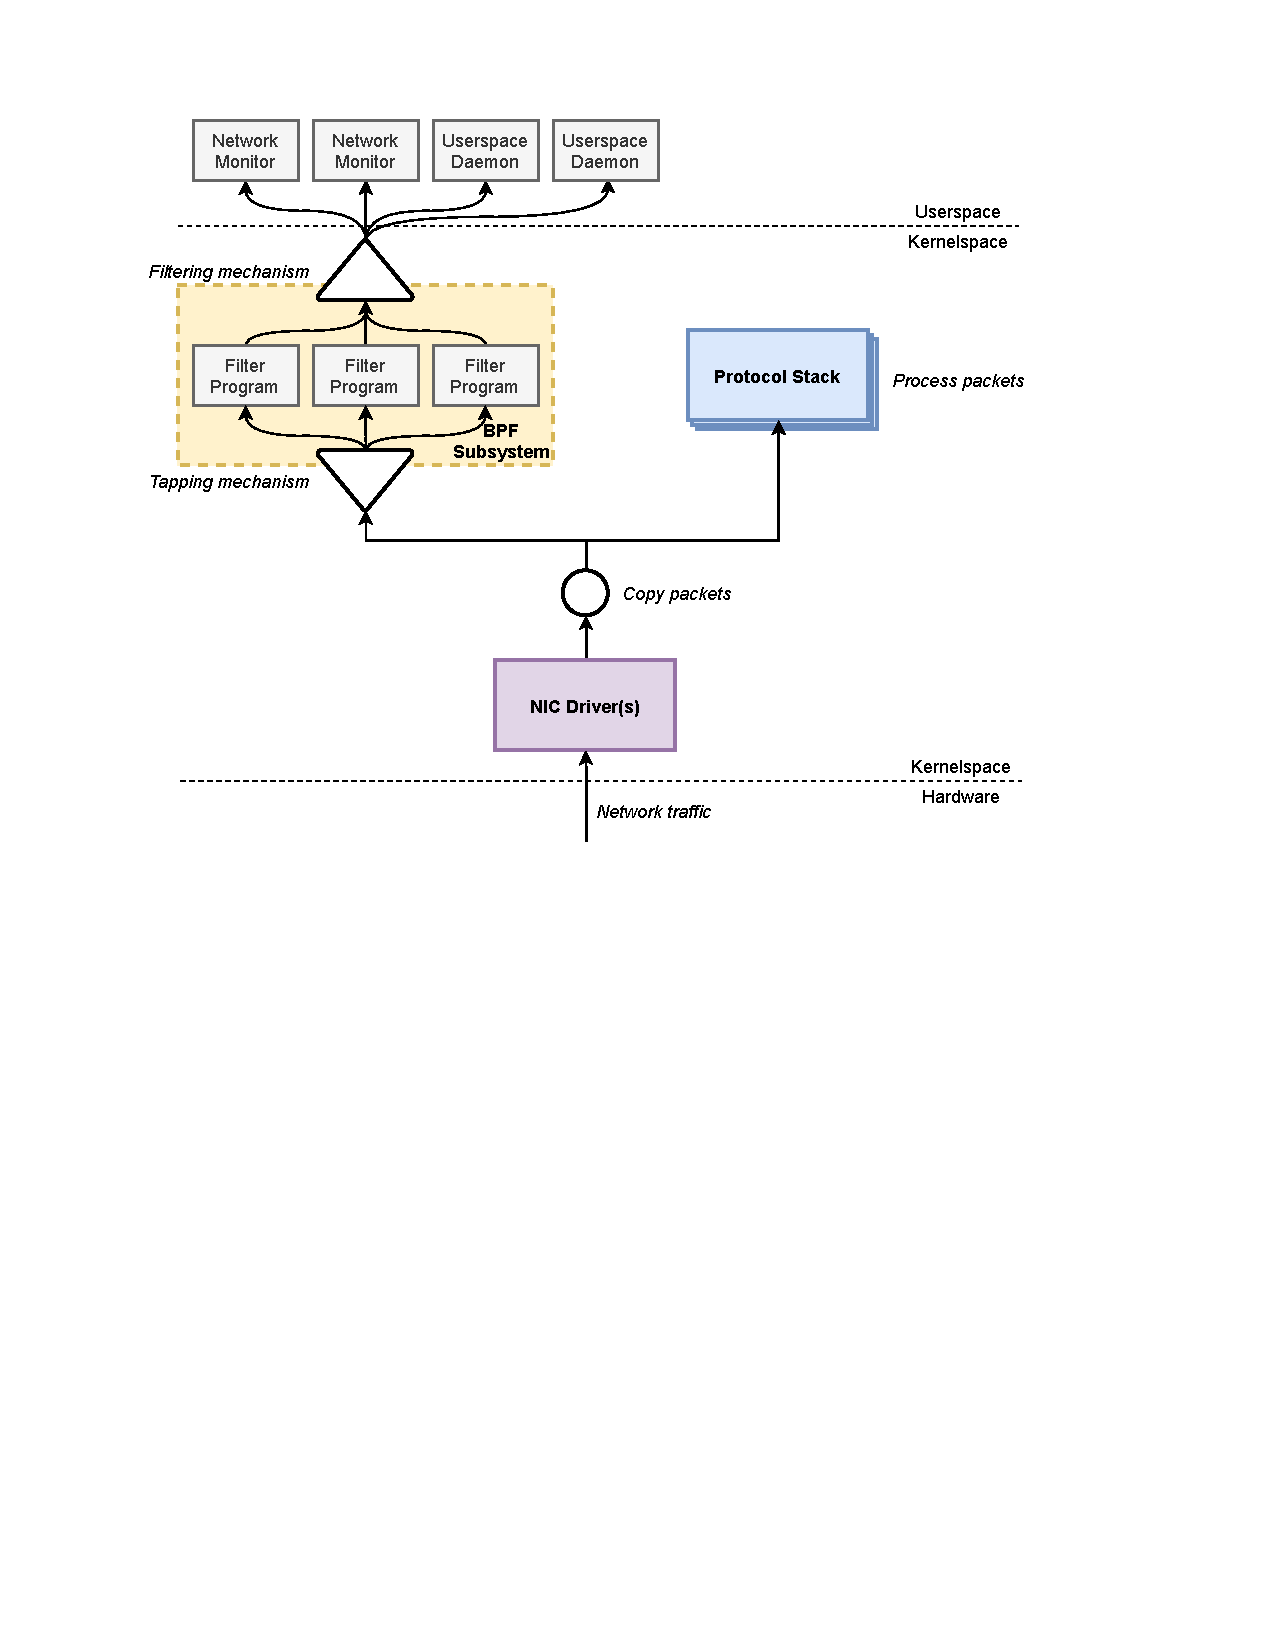
\includegraphics[width=0.8\linewidth]{figs/background/classic-bpf.pdf}
  \caption[The classic BPF architecture]{The classic BPF architecture. Adapted from McCanne and Jacobson~\cite{mccanne1993_bpf}.}%
  \label{fig:classic-bpf}
\end{figure}

Classic BPF can be divided into two major components: a \textit{tap} mechanism and a set
of one or more \textit{filter} programs. The cBPF architecture is depicted in
\Cref{fig:classic-bpf}. Classic BPF programs are expressed as a control-flow graph (CFG)
over a set of abstract registers, backed by physical registers on the CPU. The tap
mechanism hooks into packets as they enter the networking stack, copying and forwarding
them to the filters. At runtime, the filter programs walk their control-flow graph, taking
the forwarded packets as input. As output, they return a filtering decision which controls
whether or not the packet should be forwarded to userspace~\cite{mccanne1993_bpf}.

Since its original introduction in 1993, classic BPF has since been ported to a number of
Unix-like operating systems, including Linux~\cite{linux_bpf}, OpenBSD~\cite{openbsd_bpf},
and FreeBSD~\cite{freebsd_bpf}. Classic BPF forms the backbone of widely used traffic
monitoring tools, most notably tcpdump~\todo{CITE tcpdump}. In Linux, the seccomp system
call was enhanced to include classic BPF filters, allowing a user process to use classic BPF
programs to define allowlists and denylists of system calls (c.f.~\Cref{ss:seccomp-bg}).

In 2014, Alexei Starovoitov and Daniel Borkmann~\cite{starovoitov2014_ebpf} first proposed
a total overhaul of the Linux BPF engine. Their proposal, dubbed eBPF, expanded the
classic BPF execution model into a full-fledged virtual instruction set. In particular,
the extensions included a 512 byte stack, 11 registers (10 of which are general-purpose),
the ability to call a set of allowlisted kernel helper functions, the ability to attach
programs to a variety of system events, specialized data structures (called BPF maps) to
store and share data at runtime, and an in-kernel verification engine to check for program
safety. At runtime, programs can be dynamically attached to system events and are
just-in-time compiled into the native instruction set.  \Cref{fig:extended-bpf} depicts
the eBPF architecture in detail. The reader is encouraged to compare this with the classic
BPF architecture, depicted in \Cref{fig:classic-bpf}.

\begin{figure}[tbp]
  \centering
  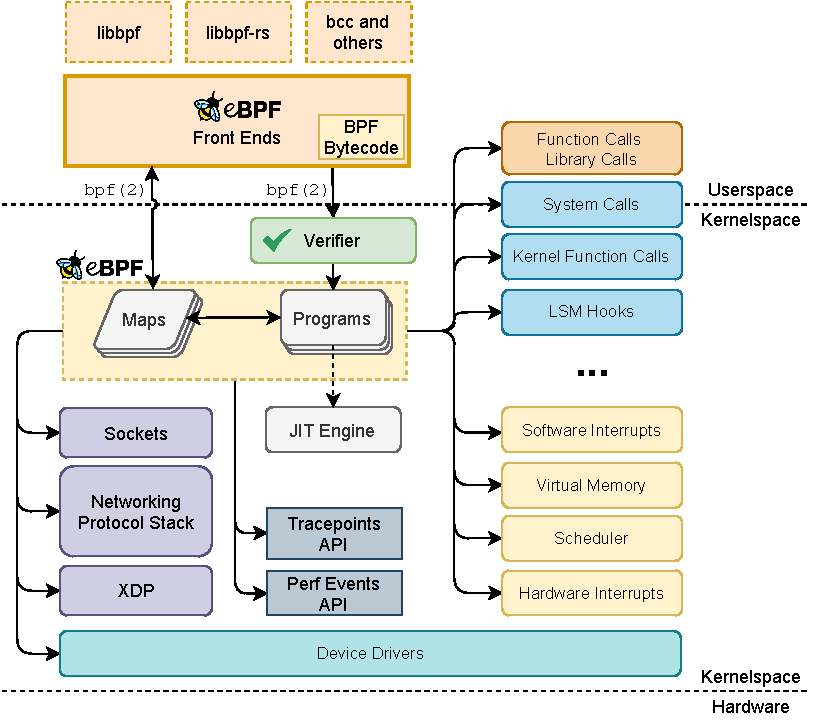
\includegraphics[width=0.8\linewidth]{figs/background/ebpf.pdf}
  \caption[The extended BPF architecture]{The extended BPF architecture. Unlike classic
  BPF, eBPF programs are JIT compiled to the native instruction set, share data using
  specialized map data structures, and can be attached to many different kinds of system
  events. All eBPF bytecode goes through a verification step before it can be loaded into
  the kernel.}%
  \label{fig:extended-bpf}
\end{figure}

While modern eBPF has very little to do with the execution model of its older cousin, some
of the properties that made classic BPF so performant still hold true today. In
particular, to notion of aggregating and processing data in kernelspace before
(optionally) handing it off to userspace is a key aspect of classic BPF that has carried
over to eBPF. What this means in practice is that eBPF programs can be used to implement
very efficient monitoring software, harnessing the performance benefits of a pure
kernelspace implementation while maintaining the flexibility of a userspace
implementation.

\subsection{eBPF Programs}%
\label{ss:bpf-programs-bg}

eBPF programs are expressed in a virtual RISC machine language called BPF bytecode.  While
it is technically possible to write BPF bytecode by hand, programs are most often compiled
from a restricted subset of the C programming language\footnote{Other languages may
eventually be used to write eBPF programs as well.  For instance, an experimental eBPF
target for the Rust programming language has recently been proposed~\todo{CITE}. The
important distinction here is that the set of all possible eBPF programs is a strict
subset of the set of all possible programs.} using the LLVM toolchain. Programs can be
loaded and attached to system events using the \texttt{bpf(2)} system call, at which point
control passes to the eBPF verifier, which checks the programs to make sure they satisfy
a set of safety constraints~\cite{starovoitov2014_ebpf, gregg2019_bpf}. In particular,
eBPF programs must consist of fewer than 1 million BPF instructions and must not call into
any kernel functions outside of the allowlisted helpers. The program is also constrained
to a 512 byte stack size; any additional memory required by the program must come from an
eBPF map (c.f.~\Cref{ss:bpf-maps-bg}). For safety, memory accesses into allocated buffers
must be properly bounds checked, pointers must be null-checked before dereferencing, and
any access to external memory (e.g.~belonging to userspace programs or to the kernel
itself) must be read-only. Since eBPF programs must provably terminate, no back-edges are
permitted in their control flow and all loops must be bounded by some fixed constant $i$
iterations.

To guard against data races, eBPF programs always hold the kernel's RCU (read-copy-update)
lock while executing, gated by the \texttt{bpf\_prog\_enter} and \texttt{bpf\_prog\_exit}
functions in the kernel~\todo{CITE kernel code}. In simple terms, the RCU lock allows
concurrent reads, except in the presence of updates,optimizing for read-mostly workloads
(i.e.~precisely the sort of workload eBPF is designed for)~\cite{mckenney2007_rcu}. This
implicitly enables BPF programs to read from many common kernel data structures without
fear of data races and simultaneously protects reads and updates to eBPF maps, at a slight
(albeit reasonable) performance penalty~\cite{mckenney2007_rcu}. In addition to holding
the RCU lock, eBPF programs are not considered \textit{preemptable} by default. In
practice, this means that eBPF programs cannot sleep and must run to termination on their
assigned core. This property, while useful in many circumstances, enforces undesirable
limitations on eBPF helpers, since it precludes any functionality that may cause the
program to sleep (e.g.~a page fault). To account for use cases where sleeping is
unavoidable, Linux 5.\todo{WHICH SUBVERSION?} introduced sleepable versions of some eBPF
program types~\todo{CITE}.

\subsubsection*{Working with the Verifier}

In practice, the restrictions imposed by the verifier mean that eBPF programs are not
\textit{Turing-complete}~\cite{gregg2019_bpf}.  This property is required, given that the
halting problem (i.e.~the decidability of program termination) is known not to be solvable
for Turing-complete programs. This notion of Turing-incompleteness means that the set of
all possible eBPF programs is a strict subset of the set of all possible C programs. While
these limitations help to ensure program safety, they also naturally restrict some
operations which \textit{may} be safe but are not strictly verifiable. To overcome the
limitations imposed by the verifier and achieve this safe-yet-unverifiable behaviour, eBPF
programmers have a few tools in their arsenal. For instance, a specific set of allowlisted
kernel helpers offers the ability to call into specific kernel functions, bypassing the
limitations imposed by the eBPF verifier. As a simple example, the
\texttt{bpf\_probe\_write\_user()} helper allows an eBPF program to write to a userspace
memory address, bypassing the read-only restrictions imposed by the verifier. While these
allowlisted helpers operate in a \textit{mostly} unrestricted context, their usage
\textit{is} restricted at the function call boundary, ensuring that the eBPF program obeys
the safety contract specified by the helper function.  Another common design pattern is
using a dummy eBPF map as a scratch buffer to reserve a larger amount of memory for the
eBPF program.  Since eBPF programs cannot sleep~\cite{gregg2019_bpf}, dynamic memory
allocation within the BPF context is impossible. These dummy maps offer a way to access
additional memory from a pool reserved at the time the map was loaded into the kernel.

\subsubsection*{eBPF Program Types and Use Cases}

Each eBPF program has a specific \textit{program type}, which determines both the set of
system events to which the program can attach and the set of allowed kernel helpers that
can be called from within the program context. Each program type roughly corresponds with
a distinct eBPF use case. For the purposes of this thesis, we will primarily be dealing
with \textit{LSM probes}, \textit{raw tracepoints}, \textit{fentry/fexit probes}, and
\textit{uprobes/uretprobes}, as they form the basis of \bpfbox{} and \bpfcontain{}'s
kernelspace implementations. \Cref{tab:program-types} summarizes the relevant program types
and their properties.

\begingroup\footnotesize
\begin{longtable}[c]{lp{4.2in}}
\caption{A selection of relevant eBPF program types for \bpfbox{} and \bpfcontain{}.}%
\label{tab:program-types}\\
  \toprule
  Program Type & Description\\
  \midrule
  \textit{LSM Probes}          & LSM probes~\cite{singh2019_krsi} attach to the kernel's LSM hooks and can be used to audit security events and make policy decisions.\\
  \textit{Raw Tracepoints}     & Raw tracepoint programs attach to a stable tracing interface exposed by the Linux kernel. Tracepoints are considered a stable API, but are more limiting than alternatives such as Kprobes or Fentry probes.\\
  \textit{Kprobes/Kretprobes}  & Kprobe programs can attach to any kernel function, by replacing the function with a trap into the BPF program. The BPF program has read-only access to the function arguments. Kretprobes work in the same way, but handle function returns instead of function calls.\\
  \textit{Fentry/Fexit Probes} & A more efficient version of Kprobes and Kretprobes that directly trampoline into the BPF program instead of trapping. These programs can also be used to modify the return value of specifically allowlisted kernel functions (e.g.~system call implementations).\\
  \textit{Uprobes/Uretprobes}  & The userspace equivalent of Kprobes and Kretprobes.\\
  \bottomrule
\end{longtable}
\endgroup

\subsubsection*{LSM Probes: Making Security Decisions with eBPF}

It is worth spending more time focusing specifically on LSM probes, as these are used
extensively in \bpfbox{} and \bpfcontain{} to enforce policy over security-sensitive
events. Introduced by KP Singh in his KRSI (Kernel Runtime Security Instrumentation)
patch~\cite{singh2019_krsi}, LSM probes define a canonical framework for attaching eBPF
programs to the Linux kernel's LSM security hooks (c.f.~\Cref{ss:linux-mac-bg}). Unlike
traditional LSMs which are implemented as static kernel modules, LSM probes are
\textit{dynamically attachable}, meaning that MAC and audit policy can be adjusted at
runtime, simply by loading a new eBPF program.  \Cref{fig:bpf-lsm} depicts how LSM probes
integrate with the LSM framework.

\begin{figure}[tbp]
  \centering
  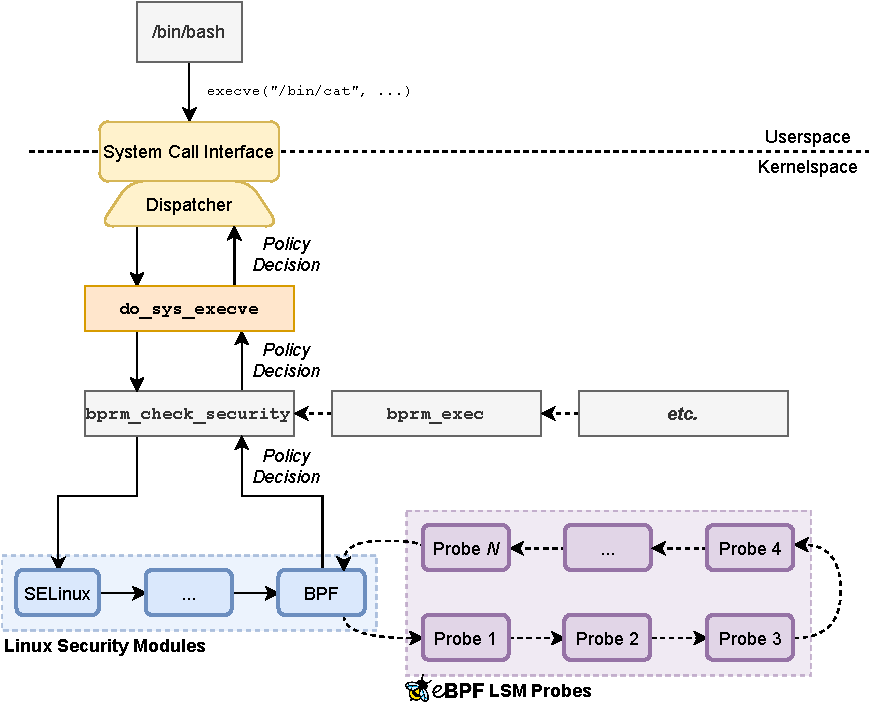
\includegraphics[width=0.8\linewidth]{figs/background/bpf-lsm.pdf}
  \caption{A simplified example of how eBPF LSM probes make policy decisions. Privileged userspace processes can attach one or more LSM probes to a given hook. When a userspace process requests a privileged operation, the kernel implicitly calls into the corresponding LSM hooks, which in turn invoke the logic associated with each LSM. A shim LSM is responsible for invoking each LSM probe, and any resulting policy decisions are taken together to arrive at a final decision. As with ordinary LSMs, the final decision is consensus-based. That is, if \textit{any LSMs} or \textit{any BPF LSM probes} disagree on a policy decision, the privileged operation is denied.}%
  \label{fig:bpf-lsm}
\end{figure}

As with other LSMs, LSM probes implement a form of mandatory access control. Each LSM
probe can be attached to one or more LSM hooks defined in the kernel. When the hook fires
(i.e.~when a task requests a privileged operation form the kernel), every attached probe
fires as part of the normal LSM pipeline. The body of the BPF program defines filtering
and audit logic, optionally accessing maps to store and query persistent state. The BPF
program then returns a security decision about whether the requested operation should be
allowed or denied.  In order for an operation to be allowed, \textit{all} other LSMs and
LSM probes must agree on the policy decision and ordinary security checks performed by the
operating system must also succeed. In other words, it is not possible to grant additional
privileges using an LSM probe.

Owing to the properties discussed earlier in this section, eBPF confers a natural
flexibility to LSM probes quite unlike that of traditional LSM-based security frameworks.
In particular, LSM probes can be attached at runtime and can cooperate with other eBPF
program types using eBPF maps (c.f.~\Cref{ss:bpf-maps-bg}). This notion of cooperating
programs presents an opportunity to design modular policy enforcement mechanisms that
operate beyond the scope of the LSM hooks framework itself.  Another key advantage of LSM
probes over traditional LSMs lies in their adoptability.  While industry actors may be
understandably reluctant to adopt \enquote{yet another out-of-tree LSM}, a security
mechanism based on eBPF does not carry the same technical baggage.  eBPF programs are safe
to use in production and can be deployed at runtime on an unmodified kernel.  This makes
eBPF a particularly attractive target for developing new security solutions.

\subsection{eBPF Maps}%
\label{ss:bpf-maps-bg}

\subsection{The BPF Type Format (BTF)}%
\label{ss:btf-bg}

\subsection{Comparing eBPF with Loadable Kernel Modules}%
\label{ss:bpf-vs-modules}

% @FIXME: This should be moved to
%\subsection{eBPF in the Wild}%
%\label{ss:ebpf-in-the-wild}
